\begin{figure}
  \begin{center}
    \psset{unit=1.5cm} % 12cm width / 8 figures = 1.5cm
    \addtolength{\subfigbottomskip}{-1.5cm}
    \multido{\ix=0+1}{13}{ % first 13
      \setcounter{subfigure}{0}
      \subfigure{
        \begin{pspicture}(-0.25,0)(-0.05,1)
          \input{common/permute\ix}
        \end{pspicture}
        \includegraphics[width=12.0cm]{primarystripes/\ix.eps}
        \rput[cl](0.05,0.5){\ix}
      }
    }
    \subfigure{ % last one with labels
      \begin{pspicture}(-0.25,0)(-0.05,1)
        \input{common/permute14}
      \end{pspicture}
      
\includegraphics[width=12.0cm]{primarystripes/14.eps}
      \rput[cl](0.05,0.5){14}
      \psset{unit=1.5cm}
      \rput[ct](-0.55,-0.3){$\frac{7\pi}{4}$}
      \rput[ct](-1.55,-0.3){$\frac{6\pi}{4}$}
      \rput[ct](-2.55,-0.3){$\frac{5\pi}{4}$}
      \rput[ct](-3.55,-0.3){$\pi$}
      \rput[ct](-4.55,-0.3){$\frac{3\pi}{4}$}
      \rput[ct](-5.55,-0.3){$\frac{\pi}{2}$}
      \rput[ct](-6.55,-0.3){$\frac{\pi}{4}$}
      \rput[ct](-7.55,-0.3){$0$}
    }
  \end{center}
  \caption{Permutations of the Monte Carlo simulation around the ring:
    intensity and phase.  Intensity values have been normalized for each frame
    while phase values normalized across the entire dataset.}
  \label{fig:clevergridlinhsv}
\end{figure}

\begin{figure}
  \begin{center}
    \psset{unit=1.5cm}
    \addtolength{\subfigbottomskip}{-1.5cm}
    \multido{\ix=0+1}{13}{
      \setcounter{subfigure}{0}
      \subfigure{
        \begin{pspicture}(-0.25,0)(-0.05,1)
          \input{common/permute\ix}
        \end{pspicture}
        % this file name sucks because of the dot, but too lazy to change
        \includegraphics[width=12.0cm]{primarystripes/\ix.-intensity.eps}
        \rput[cl](0.05,0.5){\ix}
      }
    }
    \subfigure{
      \begin{pspicture}(-0.25,0)(-0.05,1)
        \input{common/permute14}
      \end{pspicture}
      
\includegraphics[width=12.0cm]{primarystripes/14.-intensity.eps}
      \rput[cl](0.05,0.5){14}
      \psset{unit=1.5cm}
      \rput[ct](-0.55,-0.3){$\frac{7\pi}{4}$}
      \rput[ct](-1.55,-0.3){$\frac{6\pi}{4}$}
      \rput[ct](-2.55,-0.3){$\frac{5\pi}{4}$}
      \rput[ct](-3.55,-0.3){$\pi$}
      \rput[ct](-4.55,-0.3){$\frac{3\pi}{4}$}
      \rput[ct](-5.55,-0.3){$\frac{\pi}{2}$}
      \rput[ct](-6.55,-0.3){$\frac{\pi}{4}$}
      \rput[ct](-7.55,-0.3){$0$}
    }
  \end{center}
  \caption{Permutations of the Monte Carlo simulation around the ring:
    intensity only.  Intensity values have been normalized for each frame
    individually.}
  \label{fig:clevergridlinintensity}
\end{figure}


% probability distribution function around the ring
\begin{figure}
  \begin{center}
    \addtolength{\subfigbottomskip}{-1cm}
    \psset{yAxisLabel=,xAxisLabel=,yAxis=false}
    \multido{\ix=0+1}{13}{%
      \setcounter{subfigure}{0}
      \subfigure{
        \psset{unit=40.75pt}
        \begin{pspicture}(-0.25,0)(-0.05,1)
          \input{common/permute\ix}
        \end{pspicture}
        \begin{psgraph}[Dx=0.1,labels=none](0,0)(1,0.08){14cm}{1.5cm}
          \psset{fillstyle=solid,fillcolor=red}
          \input{stats/ringpdf\ix}
        \end{psgraph}
      }
    }
    \subfigure{
      \psset{unit=40.75pt}
      \begin{pspicture}(-0.25,0)(-0.05,1)
        \input{common/permute14}
      \end{pspicture}
      \begin{psgraph}[Dx=0.1](0,0)(1,0.08){14cm}{1.5cm}
        \psset{fillstyle=solid,fillcolor=red}
        \fill (0.000000,0) rectangle (0.005000,0.036111);
\fill (0.005000,0) rectangle (0.010000,0.022222);
\fill (0.010000,0) rectangle (0.015000,0.019444);
\fill (0.015000,0) rectangle (0.020000,0.027778);
\fill (0.020000,0) rectangle (0.025000,0.030556);
\fill (0.025000,0) rectangle (0.030000,0.016667);
\fill (0.030000,0) rectangle (0.035000,0.030556);
\fill (0.035000,0) rectangle (0.040000,0.019444);
\fill (0.040000,0) rectangle (0.045000,0.022222);
\fill (0.045000,0) rectangle (0.050000,0.033333);
\fill (0.050000,0) rectangle (0.055000,0.025000);
\fill (0.055000,0) rectangle (0.060000,0.011111);
\fill (0.060000,0) rectangle (0.065000,0.016667);
\fill (0.065000,0) rectangle (0.070000,0.011111);
\fill (0.070000,0) rectangle (0.075000,0.016667);
\fill (0.075000,0) rectangle (0.080000,0.019444);
\fill (0.080000,0) rectangle (0.085000,0.005556);
\fill (0.085000,0) rectangle (0.090000,0.025000);
\fill (0.090000,0) rectangle (0.095000,0.027778);
\fill (0.095000,0) rectangle (0.100000,0.011111);
\fill (0.100000,0) rectangle (0.105000,0.002778);
\fill (0.105000,0) rectangle (0.110000,0.016667);
\fill (0.110000,0) rectangle (0.115000,0.011111);
\fill (0.115000,0) rectangle (0.120000,0.019444);
\fill (0.120000,0) rectangle (0.125000,0.005556);
\fill (0.125000,0) rectangle (0.130000,0.008333);
\fill (0.130000,0) rectangle (0.135000,0.011111);
\fill (0.135000,0) rectangle (0.140000,0.011111);
\fill (0.140000,0) rectangle (0.145000,0.011111);
\fill (0.145000,0) rectangle (0.150000,0.011111);
\fill (0.150000,0) rectangle (0.155000,0.013889);
\fill (0.155000,0) rectangle (0.160000,0.011111);
\fill (0.160000,0) rectangle (0.165000,0.008333);
\fill (0.165000,0) rectangle (0.170000,0.008333);
\fill (0.170000,0) rectangle (0.175000,0.011111);
\fill (0.175000,0) rectangle (0.180000,0.011111);
\fill (0.180000,0) rectangle (0.185000,0.005556);
\fill (0.185000,0) rectangle (0.190000,0.002778);
\fill (0.190000,0) rectangle (0.195000,0.008333);
\fill (0.195000,0) rectangle (0.200000,0.011111);
\fill (0.200000,0) rectangle (0.205000,0.011111);
\fill (0.205000,0) rectangle (0.210000,0.008333);
\fill (0.210000,0) rectangle (0.215000,0.011111);
\fill (0.215000,0) rectangle (0.220000,0.011111);
\fill (0.220000,0) rectangle (0.225000,0.005556);
\fill (0.225000,0) rectangle (0.230000,0.005556);
\fill (0.230000,0) rectangle (0.235000,0.005556);
\fill (0.235000,0) rectangle (0.240000,0.005556);
\fill (0.240000,0) rectangle (0.245000,0.013889);
\fill (0.245000,0) rectangle (0.250000,0.002778);
\fill (0.250000,0) rectangle (0.255000,0.013889);
\fill (0.255000,0) rectangle (0.260000,0.011111);
\fill (0.260000,0) rectangle (0.265000,0.005556);
\fill (0.265000,0) rectangle (0.270000,0.000000);
\fill (0.270000,0) rectangle (0.275000,0.000000);
\fill (0.275000,0) rectangle (0.280000,0.002778);
\fill (0.280000,0) rectangle (0.285000,0.002778);
\fill (0.285000,0) rectangle (0.290000,0.008333);
\fill (0.290000,0) rectangle (0.295000,0.008333);
\fill (0.295000,0) rectangle (0.300000,0.005556);
\fill (0.300000,0) rectangle (0.305000,0.008333);
\fill (0.305000,0) rectangle (0.310000,0.002778);
\fill (0.310000,0) rectangle (0.315000,0.005556);
\fill (0.315000,0) rectangle (0.320000,0.005556);
\fill (0.320000,0) rectangle (0.325000,0.005556);
\fill (0.325000,0) rectangle (0.330000,0.008333);
\fill (0.330000,0) rectangle (0.335000,0.002778);
\fill (0.335000,0) rectangle (0.340000,0.005556);
\fill (0.340000,0) rectangle (0.345000,0.002778);
\fill (0.345000,0) rectangle (0.350000,0.008333);
\fill (0.350000,0) rectangle (0.355000,0.002778);
\fill (0.355000,0) rectangle (0.360000,0.005556);
\fill (0.360000,0) rectangle (0.365000,0.002778);
\fill (0.365000,0) rectangle (0.370000,0.002778);
\fill (0.370000,0) rectangle (0.375000,0.005556);
\fill (0.375000,0) rectangle (0.380000,0.000000);
\fill (0.380000,0) rectangle (0.385000,0.000000);
\fill (0.385000,0) rectangle (0.390000,0.002778);
\fill (0.390000,0) rectangle (0.395000,0.000000);
\fill (0.395000,0) rectangle (0.400000,0.008333);
\fill (0.400000,0) rectangle (0.405000,0.002778);
\fill (0.405000,0) rectangle (0.410000,0.002778);
\fill (0.410000,0) rectangle (0.415000,0.005556);
\fill (0.415000,0) rectangle (0.420000,0.002778);
\fill (0.420000,0) rectangle (0.425000,0.002778);
\fill (0.425000,0) rectangle (0.430000,0.002778);
\fill (0.430000,0) rectangle (0.435000,0.002778);
\fill (0.435000,0) rectangle (0.440000,0.000000);
\fill (0.440000,0) rectangle (0.445000,0.000000);
\fill (0.445000,0) rectangle (0.450000,0.000000);
\fill (0.450000,0) rectangle (0.455000,0.000000);
\fill (0.455000,0) rectangle (0.460000,0.005556);
\fill (0.460000,0) rectangle (0.465000,0.000000);
\fill (0.465000,0) rectangle (0.470000,0.000000);
\fill (0.470000,0) rectangle (0.475000,0.002778);
\fill (0.475000,0) rectangle (0.480000,0.005556);
\fill (0.480000,0) rectangle (0.485000,0.002778);
\fill (0.485000,0) rectangle (0.490000,0.002778);
\fill (0.490000,0) rectangle (0.495000,0.000000);
\fill (0.495000,0) rectangle (0.500000,0.000000);
\fill (0.500000,0) rectangle (0.505000,0.005556);
\fill (0.505000,0) rectangle (0.510000,0.008333);
\fill (0.510000,0) rectangle (0.515000,0.000000);
\fill (0.515000,0) rectangle (0.520000,0.008333);
\fill (0.520000,0) rectangle (0.525000,0.002778);
\fill (0.525000,0) rectangle (0.530000,0.002778);
\fill (0.530000,0) rectangle (0.535000,0.000000);
\fill (0.535000,0) rectangle (0.540000,0.000000);
\fill (0.540000,0) rectangle (0.545000,0.000000);
\fill (0.545000,0) rectangle (0.550000,0.002778);
\fill (0.550000,0) rectangle (0.555000,0.002778);
\fill (0.555000,0) rectangle (0.560000,0.000000);
\fill (0.560000,0) rectangle (0.565000,0.000000);
\fill (0.565000,0) rectangle (0.570000,0.005556);
\fill (0.570000,0) rectangle (0.575000,0.002778);
\fill (0.575000,0) rectangle (0.580000,0.000000);
\fill (0.580000,0) rectangle (0.585000,0.002778);
\fill (0.585000,0) rectangle (0.590000,0.000000);
\fill (0.590000,0) rectangle (0.595000,0.002778);
\fill (0.595000,0) rectangle (0.600000,0.000000);
\fill (0.600000,0) rectangle (0.605000,0.002778);
\fill (0.605000,0) rectangle (0.610000,0.000000);
\fill (0.610000,0) rectangle (0.615000,0.002778);
\fill (0.615000,0) rectangle (0.620000,0.002778);
\fill (0.620000,0) rectangle (0.625000,0.000000);
\fill (0.625000,0) rectangle (0.630000,0.000000);
\fill (0.630000,0) rectangle (0.635000,0.002778);
\fill (0.635000,0) rectangle (0.640000,0.002778);
\fill (0.640000,0) rectangle (0.645000,0.002778);
\fill (0.645000,0) rectangle (0.650000,0.005556);
\fill (0.650000,0) rectangle (0.655000,0.000000);
\fill (0.655000,0) rectangle (0.660000,0.000000);
\fill (0.660000,0) rectangle (0.665000,0.000000);
\fill (0.665000,0) rectangle (0.670000,0.002778);
\fill (0.670000,0) rectangle (0.675000,0.000000);
\fill (0.675000,0) rectangle (0.680000,0.000000);
\fill (0.680000,0) rectangle (0.685000,0.000000);
\fill (0.685000,0) rectangle (0.690000,0.002778);
\fill (0.690000,0) rectangle (0.695000,0.000000);
\fill (0.695000,0) rectangle (0.700000,0.000000);
\fill (0.700000,0) rectangle (0.705000,0.000000);
\fill (0.705000,0) rectangle (0.710000,0.000000);
\fill (0.710000,0) rectangle (0.715000,0.000000);
\fill (0.715000,0) rectangle (0.720000,0.002778);
\fill (0.720000,0) rectangle (0.725000,0.000000);
\fill (0.725000,0) rectangle (0.730000,0.000000);
\fill (0.730000,0) rectangle (0.735000,0.000000);
\fill (0.735000,0) rectangle (0.740000,0.002778);
\fill (0.740000,0) rectangle (0.745000,0.000000);
\fill (0.745000,0) rectangle (0.750000,0.000000);
\fill (0.750000,0) rectangle (0.755000,0.000000);
\fill (0.755000,0) rectangle (0.760000,0.002778);
\fill (0.760000,0) rectangle (0.765000,0.002778);
\fill (0.765000,0) rectangle (0.770000,0.002778);
\fill (0.770000,0) rectangle (0.775000,0.000000);
\fill (0.775000,0) rectangle (0.780000,0.000000);
\fill (0.780000,0) rectangle (0.785000,0.000000);
\fill (0.785000,0) rectangle (0.790000,0.000000);
\fill (0.790000,0) rectangle (0.795000,0.000000);
\fill (0.795000,0) rectangle (0.800000,0.000000);
\fill (0.800000,0) rectangle (0.805000,0.000000);
\fill (0.805000,0) rectangle (0.810000,0.000000);
\fill (0.810000,0) rectangle (0.815000,0.000000);
\fill (0.815000,0) rectangle (0.820000,0.000000);
\fill (0.820000,0) rectangle (0.825000,0.000000);
\fill (0.825000,0) rectangle (0.830000,0.000000);
\fill (0.830000,0) rectangle (0.835000,0.000000);
\fill (0.835000,0) rectangle (0.840000,0.000000);
\fill (0.840000,0) rectangle (0.845000,0.000000);
\fill (0.845000,0) rectangle (0.850000,0.000000);
\fill (0.850000,0) rectangle (0.855000,0.000000);
\fill (0.855000,0) rectangle (0.860000,0.000000);
\fill (0.860000,0) rectangle (0.865000,0.000000);
\fill (0.865000,0) rectangle (0.870000,0.000000);
\fill (0.870000,0) rectangle (0.875000,0.000000);
\fill (0.875000,0) rectangle (0.880000,0.000000);
\fill (0.880000,0) rectangle (0.885000,0.000000);
\fill (0.885000,0) rectangle (0.890000,0.000000);
\fill (0.890000,0) rectangle (0.895000,0.002778);
\fill (0.895000,0) rectangle (0.900000,0.000000);
\fill (0.900000,0) rectangle (0.905000,0.000000);
\fill (0.905000,0) rectangle (0.910000,0.000000);
\fill (0.910000,0) rectangle (0.915000,0.000000);
\fill (0.915000,0) rectangle (0.920000,0.000000);
\fill (0.920000,0) rectangle (0.925000,0.000000);
\fill (0.925000,0) rectangle (0.930000,0.002778);
\fill (0.930000,0) rectangle (0.935000,0.000000);
\fill (0.935000,0) rectangle (0.940000,0.000000);
\fill (0.940000,0) rectangle (0.945000,0.000000);
\fill (0.945000,0) rectangle (0.950000,0.000000);
\fill (0.950000,0) rectangle (0.955000,0.000000);
\fill (0.955000,0) rectangle (0.960000,0.000000);
\fill (0.960000,0) rectangle (0.965000,0.000000);
\fill (0.965000,0) rectangle (0.970000,0.000000);
\fill (0.970000,0) rectangle (0.975000,0.000000);
\fill (0.975000,0) rectangle (0.980000,0.002778);
\fill (0.980000,0) rectangle (0.985000,0.000000);
\fill (0.985000,0) rectangle (0.990000,0.000000);
\fill (0.990000,0) rectangle (0.995000,0.000000);
\fill (0.995000,0) rectangle (1.000000,0.002778);

      \end{psgraph}
    }
  \end{center}
  \caption{Probability distribution function, plotted here as a histogram, of
    the normalized binned averaged intensities of weirdospace images around the
    ring.}
  \label{fig:intensitypdf}
\end{figure}

% distribution of the numbers of scatterers
\begin{figure}
  \begin{center}
    \addtolength{\subfigbottomskip}{-1cm}
    \psset{yAxisLabel=,xAxisLabel=,yAxis=false}
    \multido{\ix=0+1}{13}{%
      \setcounter{subfigure}{0}
      \subfigure{
        \psset{unit=40.75pt}
        \begin{pspicture}(-0.25,0)(-0.05,1)
          \input{common/permute\ix}
        \end{pspicture}
        \begin{psgraph}[Dx=1,labels=none](1,0)(19,0.6){14cm}{1.5cm}
          \psset{fillstyle=solid,fillcolor=red}
          \input{stats/nhist\ix}
          \psset{fillstyle=solid,fillcolor=blue}
          \input{stats/snhist\ix}
        \end{psgraph}
      }
    }
    \subfigure{
      \psset{unit=40.75pt}
      \begin{pspicture}(-0.25,0)(-0.05,1)
        \input{common/permute14}
      \end{pspicture}
      \begin{psgraph}[Dx=1,labels=none](1,0)(19,0.6){14cm}{1.5cm}
        \psset{fillstyle=solid,fillcolor=red}
        \fill (1.000000,0) rectangle (2.000000,0.000000);
\fill (2.000000,0) rectangle (3.000000,0.061260);
\fill (3.000000,0) rectangle (4.000000,0.065566);
\fill (4.000000,0) rectangle (5.000000,0.177652);
\fill (5.000000,0) rectangle (6.000000,0.297484);
\fill (6.000000,0) rectangle (7.000000,0.241226);
\fill (7.000000,0) rectangle (8.000000,0.112900);
\fill (8.000000,0) rectangle (9.000000,0.034768);
\fill (9.000000,0) rectangle (10.000000,0.007614);
\fill (10.000000,0) rectangle (11.000000,0.001324);
\fill (11.000000,0) rectangle (12.000000,0.000178);
\fill (12.000000,0) rectangle (13.000000,0.000024);
\fill (13.000000,0) rectangle (14.000000,0.000004);
\fill (14.000000,0) rectangle (15.000000,0.000000);
\fill (15.000000,0) rectangle (16.000000,0.000000);
\fill (16.000000,0) rectangle (17.000000,0.000000);
\fill (17.000000,0) rectangle (18.000000,0.000000);
\fill (18.000000,0) rectangle (19.000000,0.000000);
\fill (19.000000,0) rectangle (20.000000,0.000000);

        \input{stats/snhist14}
        \multido{\ry=1.5+1,\ix=1+1}{19}{%
          \rput[t](\ry,-0.15){\ix}
        }
      \end{psgraph}
    }
  \end{center}
  \caption{Histogram showing the normalized distribution of scattering
    paths having visited a certain number of scattering sites.  All
    paths are shown in red, and the proportion of those paths including the tip
    in some way are shown in blue.}
  \label{fig:scatterhist}
\end{figure}

\begin{figure}
  \begin{center}
    \psset{xunit=0.10cm,yunit=1cm}
    \psset{yAxisLabel=,xAxisLabel=,yAxis=false}
    \addtolength{\subfigbottomskip}{-1cm}
    %\psset{yAxisLabel=intensity (a.u),xAxisLabel=ring
    %angle (degrees),llx=-.5cm,lly=-1.5cm,ury=0.5cm,
    %xAxisLabelPos={c,-0.2},yAxisLabelPos={-22,c}}
    \multido{\ix=0+1}{13}{%
      \subfigure{
        \psset{unit=40.75pt}
        \begin{pspicture}(-0.25,0)(-0.05,1)
          \input{common/permute\ix}
        \end{pspicture}
        \readdata{\dataa}{contrast/ring\ix.dat}
        \readdata{\datab}{contrast/cring\ix.dat}
        \begin{psgraph}[Dx=20,Dy=10.2,Oy=0,labels=none](0,0)(360,1.2){14.0cm}{1.5cm}
          \listplot[linecolor=red,showpoints=true,dotstyle=+]{\dataa}
          \listplot[linecolor=blue,showpoints=true,dotstyle=+]{\datab}
        \end{psgraph}
      }
    }
    \subfigure{
      \psset{unit=40.75pt}
      \begin{pspicture}(-0.25,0)(-0.05,1)
        \input{common/permute14}
      \end{pspicture}
      \readdata{\dataa}{contrast/ring14.dat}
      \readdata{\datab}{contrast/cring14.dat}
      \pstScalePoints(1,1){180 div}{}
      \begin{psgraph}[dx=0.25,Dy=10.2,Oy=0,labels=x,trigLabels,trigLabelBase=4](0,0)(2,1.2){14.0cm}{1.5cm}
        \listplot[linecolor=red,showpoints=true,dotstyle=+]{\dataa}
        \listplot[linecolor=blue,showpoints=true,dotstyle=+]{\datab}
      \end{psgraph}
    }
  \end{center}
  \caption{Normalized intensity (red) and normalized contrast (blue) of
    weirdospace images around the ring.  Contrast here is defined as the
    average of the top \SI{1}{\percent} minus the average of the bottom
    \SI{1}{\percent} of the intensity values.
  }
  \label{fig:intensitycontrast}
\end{figure}

% vortex guys
\begin{figure}
  \begin{center}
    \readdata{\dataa}{vortex/zoom_intensity.dat}
    \readdata{\datab}{vortex/zoom_contrast.dat}
    \psset{xunit=0.10cm,yunit=1cm}

    \begin{pspicture}(-10,-10)(10,10)
      \rput{90}(33,0){
        \psset{xAxisLabel=,yAxisLabel=,llx=-.5cm,lly=-1cm,ury=0.5cm, xAxisLabelPos={c,-1},yAxisLabelPos={-7,c}}
        \begin{psgraph}[Dx=20,Dy=0.1,Oy=0.8](300,0.8)(400,1.20){20.0cm}{5cm}
          \listplot[linecolor=red,showpoints=true,dotstyle=+]{\datab}
          \psplot[linestyle=dashed,linecolor=green]{300}{400}{1}
        \end{psgraph}
      }
      \rput{90}(-30,0){
        \psset{xAxisLabel=,yAxisLabel=,llx=-.5cm, xAxisLabelPos={c,-1},yAxisLabelPos={-7,c}}
        \begin{psgraph}[Dx=20,Dy=5,Oy=5](300,5)(400,50){20.0cm}{5cm}
          \listplot[linecolor=red,showpoints=true,dotstyle=+]{\dataa}
          \psplot[linestyle=dashed,linecolor=green]{300}{400}{12}
        \end{psgraph}
      }

      \rput{90}(0,0){
        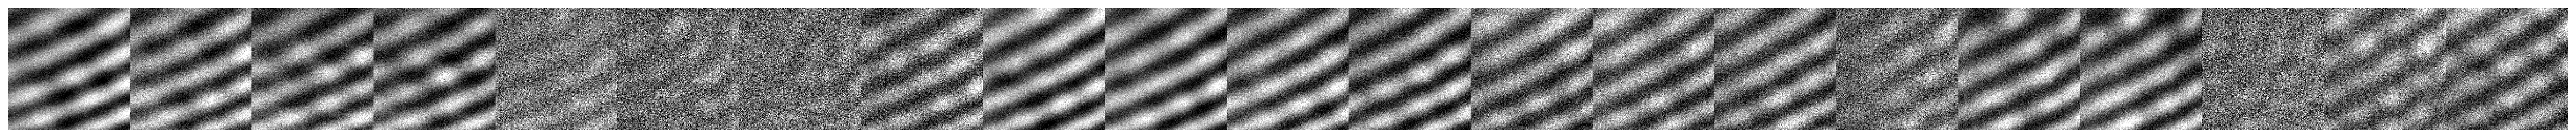
\includegraphics[width=21.1cm]{vortex/sbs.eps}
      }

      \rput[l]{90}(-45,8.5){\parbox{5cm}{
          \Rnode{A}{} \hskip 0.5cm \Rnode{B}{  Intensity} \ncline[linecolor=red]{A}{B} \\
        }}

      \rput[l]{90}(10,8.5){\parbox{5cm}{
          \Rnode{A}{} \hskip 0.5cm \Rnode{B}{  Contrast} \ncline[linecolor=red]{A}{B} \\
        }}

      \rput[c]{90}(65,0){ring angle (a.u)}

    \end{pspicture}
  \end{center}
  \caption{Intensity and contrast in a ``vortex'' area.  Contrast is defined
    here as the ratio of the range (average of the top \SI{1}{\percent} minus
    the average of the bottom \SI{1}{\percent} of the intensity values) divided
    by the mean intensity.  Note that in certain dark areas of the ring you can
    still have as much contrast as in some of the brightest places.
    The green dashed line in the intensity plot is the noise threshold. }
  \label{fig:vortexcontrast}
\end{figure}

\begin{figure}
  \begin{center}
    \psset{xunit=1.6711cm,yunit=4cm}
    \readdata{\dataa}{primarystripes/cone5.txt}
    \readdata{\datab}{primarystripes/acone5.dat}
    \begin{pspicture}(0,0)(6.2832,1.5)
      \psaxes[trigLabelBase=2,dx=\psPiH,trigLabels,Dy=0.2]{-}(0,0)(6.2832,1.5)
      \listplot[linecolor=red,plotstyle=dots,dotstyle=o]{\dataa}
      \psclip{\psframe[linestyle=none](0,0)(6,1.4)}
      \listplot[linecolor=blue]{\datab}
      \endpsclip
    \end{pspicture}
  \end{center}
  \caption{Primary stripe angle as a function position around the ring:
    experiment and theory.  This data was taken from Bert's thesis.}
  \label{fig:bertconeangle}
\end{figure}


